\section{Rešitev}

Najprej si poglejmo če sploh znamo kaj izrisat numerično.

\begin{figure}[h]
    \centering
    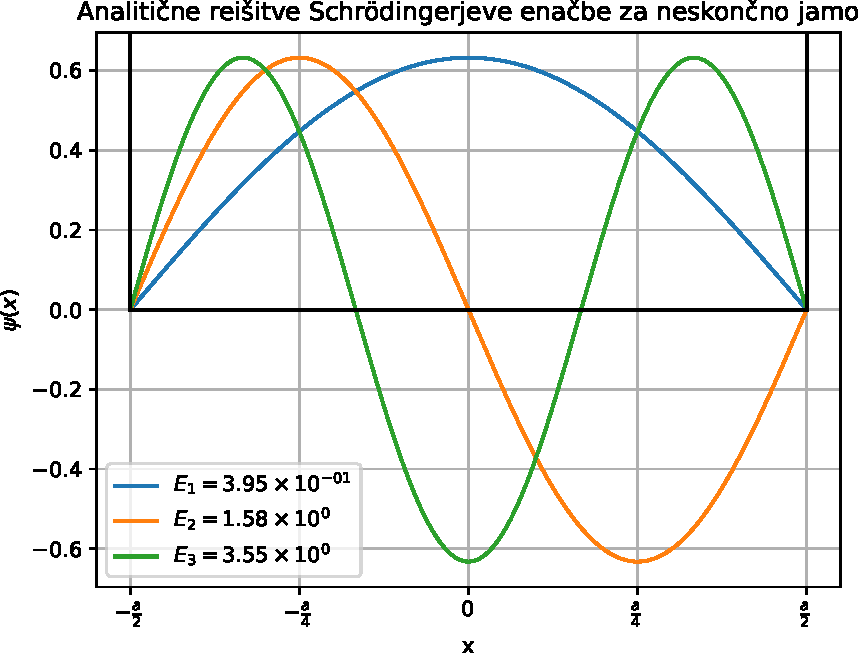
\includegraphics[width=0.415\textwidth]{pdfs/neskoncna_jama_analiticno.pdf}
    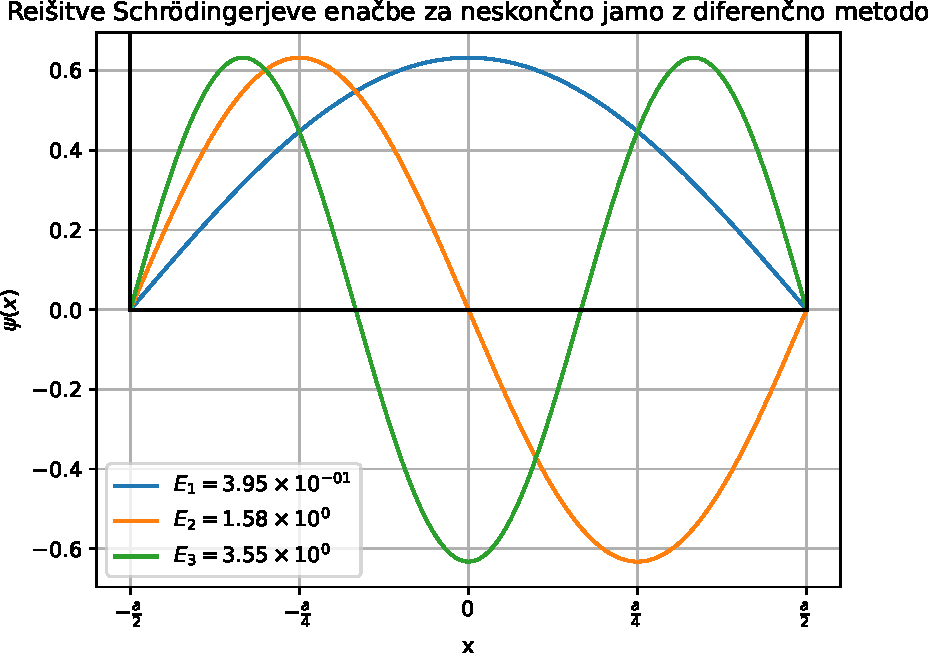
\includegraphics[width=0.45\textwidth]{pdfs/neskoncna_jama_num.pdf}
    \caption{Primerjava analitične in numerične rešitve za neskončno globoko kvadratno jamo.}
\end{figure}
Vidimo, da neki znamo. Poglejmo si še  strelsko metodo.
\begin{figure}[h]
    \centering
    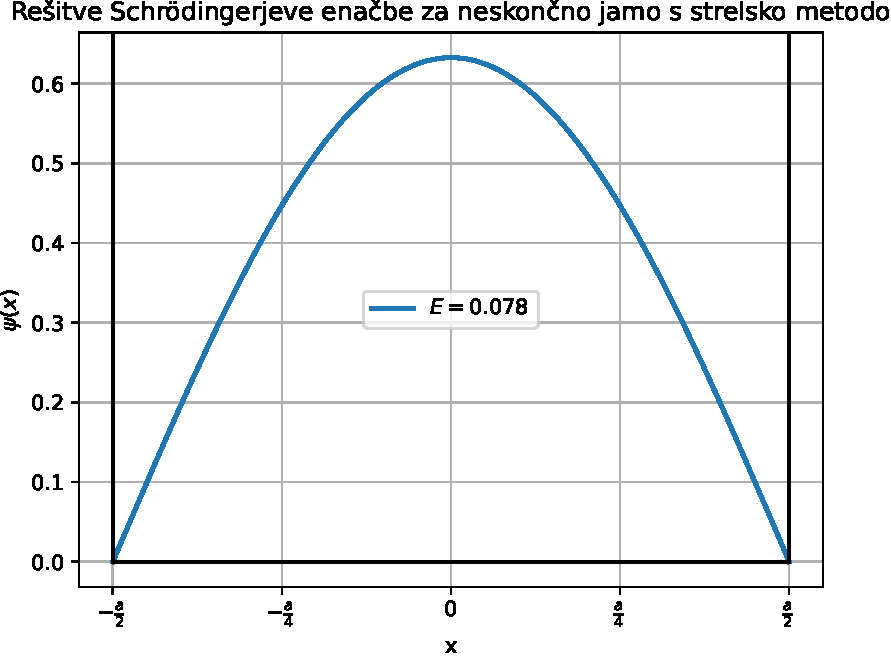
\includegraphics[width=0.5\textwidth]{pdfs/neskoncna_jama_strelska.pdf}
    \caption{Strelska metoda za neskončno globoko jamo, kjer vidimo tudi lastno vrednost.}
\end{figure}
Lastna vrdnost se ujema. 
\newpage
Poglejmo kako se obnaša strelska metoda za različne fiksne energije.
\begin{figure}[h]
    \centering
    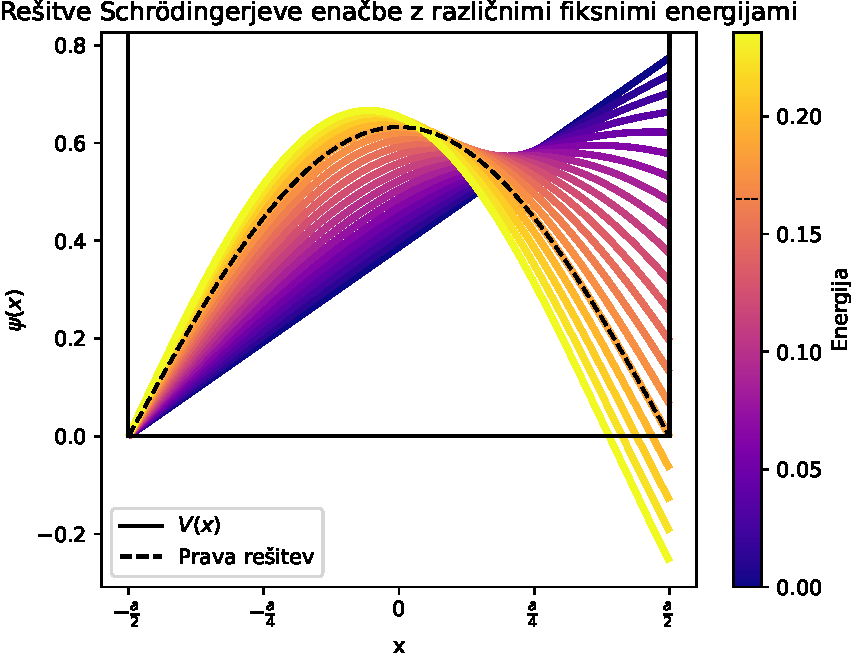
\includegraphics[width=\textwidth]{pdfs/neskoncna_jama_strelska_vec.pdf}
    \caption{Strelska metoda za neskončno globoko jamo, z različnimi fiksnimi energijami.}
\end{figure}
Še kako se absolutna napaka odvisna od pozicije in stanja.
\newpage
\begin{figure}[h]
    \centering
    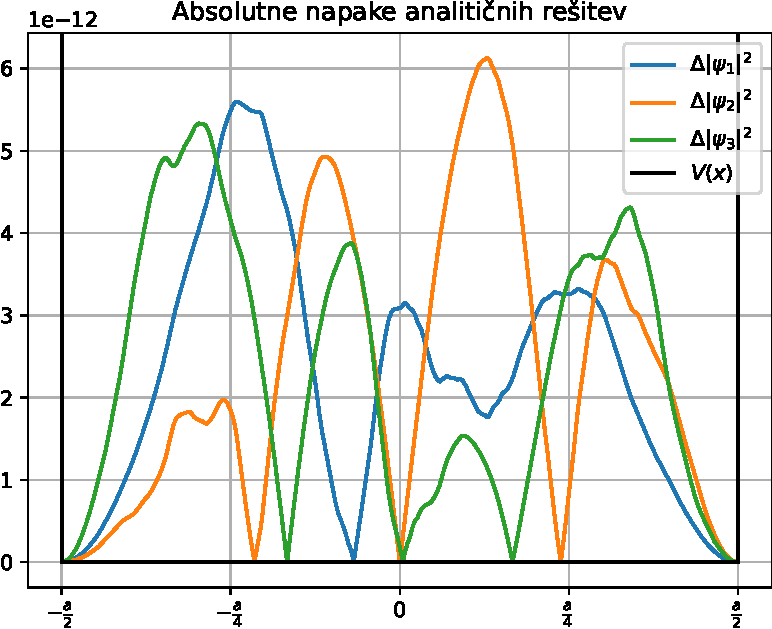
\includegraphics[width=0.6\textwidth]{pdfs/neskoncna_jama_absolutne.pdf}
    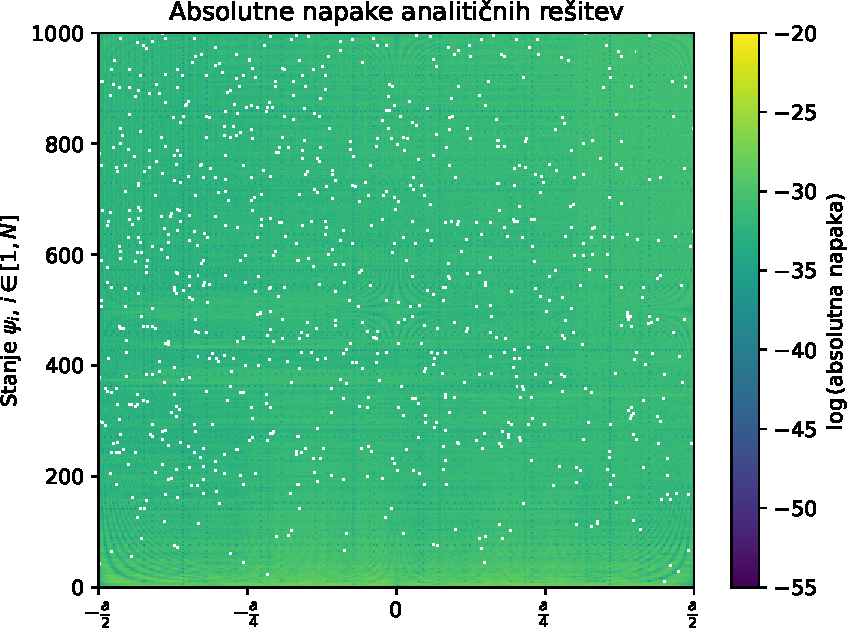
\includegraphics[width=0.7\textwidth]{pdfs/neskoncna_jama_absolutne_barva.pdf}

    \caption{Absolutna napaka diferenčne metode za neskončno globoko jamo.}
\end{figure}
\newpage
Nazadnje še lastne vrednosti in lastni vektorji za končno jamo.
\begin{figure}
    \centering
    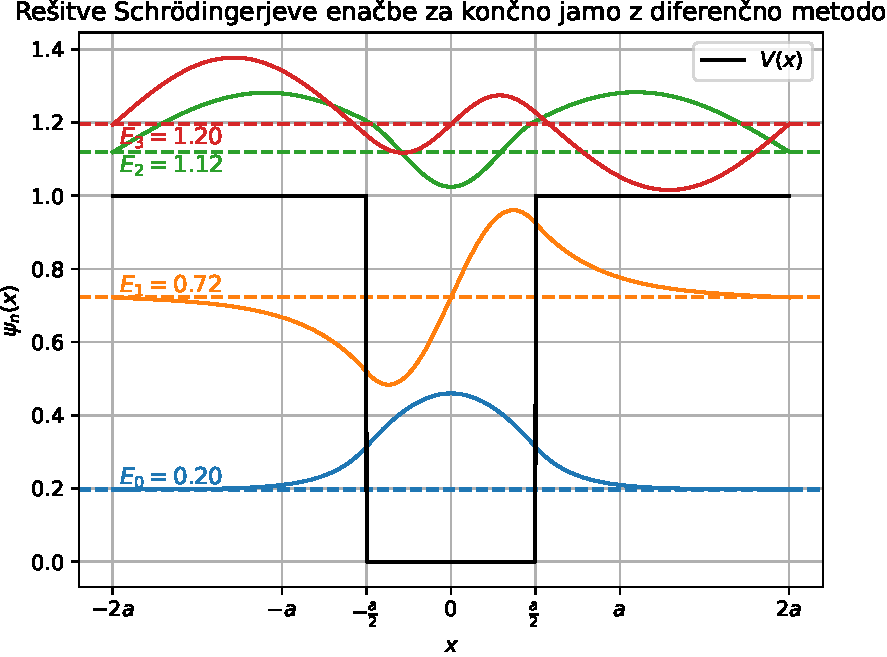
\includegraphics[width=\textwidth]{pdfs/jama.pdf}
    \caption{Lastne vrednosti in lastni vektorji za končno globoko jamo.}
\end{figure}